\documentclass[11pt,reqno]{amsart}

\usepackage[T1]{fontenc}
\usepackage[utf8]{inputenc}
\usepackage{lmodern}
\usepackage{amsmath,amssymb,amsthm}
\usepackage{booktabs,array,graphicx,microtype}
\usepackage[margin=1in]{geometry}
\usepackage[numbers,sort&compress]{natbib}
\usepackage[hidelinks]{hyperref}

\newtheorem{theorem}{Theorem}
\newtheorem{lemma}[theorem]{Lemma}
\newtheorem{proposition}[theorem]{Proposition}
\newtheorem{corollary}[theorem]{Corollary}

\theoremstyle{definition}
\newtheorem{definition}[theorem]{Definition}
\newtheorem{problem}[theorem]{Open Problem}

\theoremstyle{remark}
\newtheorem{remark}[theorem]{Remark}

\newcommand{\E}{\mathbb{E}}
\newcommand{\Var}{\operatorname{Var}}
\newcommand{\Cov}{\operatorname{Cov}}
\newcommand{\Tr}{\operatorname{Tr}}
\newcommand{\Jbar}{\overline{J}}
\newcommand{\F}{\mathcal{F}}

\title[Overbudget Haar-Purity Subsystem Designs]{Overbudget Haar-Purity Subsystem Designs Beyond the Quadratic Threshold}

\author{Thijs Missiaen}
\address{Independent Researcher, Bruges, Belgium}
\email{thijs.missiaen@gmail.com}
\urladdr{https://orcid.org/0009-0007-3678-0810}

\date{November 2026}

\begin{document}

\begin{abstract}
For an even number $n = 2k$ of $d$-dimensional quantum subsystems, we resolve the extremal geometry of the complex-Haar subsystem-purity variance across arbitrary cut budgets $1 \le m \le M_n = \frac{1}{2}\binom{2k}{k}$ and all integer local dimensions $d \ge 2$.
We prove an exact spectral formula for the folded Johnson association scheme $\Jbar(2k,k)$, showing that quadratic supersaturated-design surrogates ($E(s^2)$) agree identically with Haar optimization for $n \le 10$ but diverge strictly for every $n \ge 12$, where $S(5,6,12)/\mathbb{Z}_2$ governs a sharp Delsarte linear-programming phase transition at $m=66$ and yields dimension-uniform global optima at $m \in \{11,22,55,66,132,330,396,462\}$.
For fixed $d \ge 2$ as $n \to \infty$, we establish an exact Parseval sandwich proving that $B_{n,d}(m) = \frac{d+1}{2\sqrt{d}}\,m^2\bigl(\frac{d+1}{2}\bigr)^n(1+o(1))$ whenever $m/M_n \gg \sqrt{n}\bigl(\frac{d}{d+1}\bigr)^n$, with an exponentially small relative gap at any fixed cut density.
\end{abstract}

\maketitle

\section{Introduction}

Let $\mathcal{H} = (\mathbb{C}^d)^{\otimes n}$ denote an $n$-party quantum system of even size $n = 2k$ and local dimension $d \ge 2$ ($D = d^n$). For a pure state $|\psi\rangle \in \mathcal{H}$ and a balanced bipartition $A \subset [n] := \{0,1,\dots,n-1\}$ ($|A|=k$), the subsystem purity $P_A(\psi) = \Tr(\rho_A(\psi)^2)$ of $\rho_A(\psi) = \Tr_{A^c}(|\psi\rangle\langle\psi|)$ depends only on $\{A, A^c\}$. Let $\Jbar(2k,k)$ denote the $M_n = \frac{1}{2}\binom{2k}{k}$ complementary pairs of balanced cuts, canonically indexed by $k$-subsets containing $0$. For a cut family $\F = \{A_1,\dots,A_m\} \subseteq \Jbar(2k,k)$, we study the complex-Haar variance of $\overline{P}_{\F}(\psi) = \frac{1}{m}\sum_{a=1}^m P_{A_a}(\psi)$.

Write $g_{ab} := 4|A_a \cap A_b| - n \in [-n, n]$ for the overlap discrepancy of canonical representatives, and set
\begin{equation}\label{eq:S_def}
h_{n,d}(g) := d^{(n-g)/2} + d^{(n+g)/2}, \qquad S_{n,d}(\F) := \sum_{1 \le a < b \le m} h_{n,d}(g_{ab}), \qquad Q(\F) := \sum_{1 \le a < b \le m} g_{ab}^2,
\end{equation}
and $B_{n,d}(m) := \min_{|\F|=m} S_{n,d}(\F)$. At the Hadamard budget $m = n$, $\F$ forms an $n \times n$ binary design whose $E(s^2)$ criterion~\cite{BoothCox1962} is proportional to $Q(\F)$; for $m \le n-1$ when $n$ is a Hadamard order, pairwise orthogonal cuts ($g_{ab}=0$) exist. At $m = n$ and $n \in \{6,8,10,12,14,16\}$, Shiroshita~\cite{Shiroshita2026} established the dimension-uniform global minimum of $\Var(\overline{P}_{\F})$ via an exact Haar reduction (Lemma~\ref{lem:haar_cov}), a $0$--$4$ quadratic floor ($Q(\F) \ge \frac{n^3}{2(n-1)}$ when $4 \mid n$), and a scalar minorant on $|g_{ab}| \in \{0,4\}$. In the \emph{overbudget regime} $m > n$, orthogonal cuts are exhausted, outer adjacent pairs ($|g_{ab}| = n-4$) eventually become unavoidable, and the $0$--$4$ minorant fails.

We classify Haar-purity subsystem designs across all budgets $1 \le m \le M_n$ and all even $n \ge 6$ via the folded Johnson association scheme $\Jbar(2k,k)$~\cite{Delsarte1973,BannaiIto1984}, beginning with an exact alphabet dichotomy.

\begin{theorem}[Alphabet dichotomy and $E(s^2)$-versus-Haar separation]\label{thm:separation}
Let $n = 2k \ge 6$ be even and $d \ge 2$ be an integer.
\begin{enumerate}
\item[(a)] \emph{Collapse for $n \le 10$.} For every $n \in \{6,8,10\}$, the off-diagonal overlap alphabet $\{|g_{ab}| : a \ne b\}$ has cardinality at most $2$. Consequently, $h_{n,d}(g) = \alpha_{n,d} + \beta_{n,d} g^2$ on all off-diagonal pairs with explicit $\beta_{n,d} > 0$, so minimizing $S_{n,d}(\F)$ is identically equivalent to minimizing $Q(\F)$ for every $1 \le m \le M_n$ and every $d \ge 2$.
\item[(b)] \emph{Failure of quadratic minorization for $n \ge 12$.} For every even $n \ge 12$, the off-diagonal alphabet $\{|g_{ab}| : a \ne b\}$ has cardinality $\lfloor k/2 \rfloor \ge 3$, and for every real $d > 1$ the function $x \mapsto h_{n,d}(\sqrt{x})$ is strictly convex on $[0,\infty)$. Hence the affine secant through the two innermost off-diagonal levels strictly underestimates $h_{n,d}(g)$ at every outer overlap level $|g|$.
\item[(c)] \emph{Certified separation families.} At $n=12$ ($m \in \{20,40,50,60,140,220\}$) and $n=14$ ($m \in \{40,80,140\}$), the explicit canonical-cut families $\F_Q, \F_H \subset \Jbar(2k,k)$ archived in \url{scripts/certificates_data.json} satisfy $Q(\F_Q) \le Q(\F_H)$ while $S_{n,d}(\F_Q) > S_{n,d}(\F_H)$ simultaneously for \emph{all} integers $d \ge 2$; in particular, at $n=12$, $m=60$, $Q(\F_Q) = 19{,}344 < 19{,}440 = Q(\F_H)$ yet $S_{12,10}(\F_Q)/S_{12,10}(\F_H) > 8.43$.
\end{enumerate}
\end{theorem}

The mechanism driving both Theorem~\ref{thm:separation} and global overbudget optimality is an exact diagonalization of the folded Haar kernel $H_{\mathrm{fold}}(A,B) := h_{n,d}(g_{AB})$ on $\Jbar(2k,k)$. In the association scheme $\Jbar(2k,k)$, pairs $\{A,B\}$ are partitioned by folded distance $\delta \in \{0,1,\dots,\lfloor k/2 \rfloor\}$ ($|g| = n - 4\delta$) into adjacency matrices $A_\delta$ of valency $\overline{v}_\delta$, where $\overline{v}_0 = 1$, $\overline{v}_\delta = \binom{k}{\delta}^2$ for $1 \le \delta < k/2$, and $\overline{v}_{k/2} = \frac{1}{2}\binom{k}{k/2}^2$ when $k$ is even. The Bose--Mesner algebra decomposes $\mathbb{R}^{\Jbar(2k,k)}$ into orthogonal eigenspaces $\bigoplus_{i \ge 0,\, i\text{ even}}^k V_i$ of dimensions $m_i = \binom{n}{i} - \binom{n}{i-1}$ (with $\binom{n}{-1}=0$), orthogonal projectors $\Pi_i$, and folded Eberlein eigenvalues $\overline{P}_{i,\delta}$ ($A_\delta|_{V_i} = \overline{P}_{i,\delta} I$).

\begin{theorem}[Spectral theorem for the folded Haar kernel]\label{thm:spectral}
For every even $n = 2k \ge 4$, every real $d > 1$, and every even index $0 \le i \le k$, the eigenvalue $\Lambda_i(n,d) := \sum_{\delta=0}^{\lfloor k/2 \rfloor} h_{n,d}(n - 4\delta)\,\overline{P}_{i,\delta}$ of $H_{\mathrm{fold}}$ on $V_i$ is given identically by
\begin{equation}\label{eq:lambda_closed}
\Lambda_i(n,d) = \sum_{r=i}^{k} (d^2 - 1)^r \binom{k-i}{k-r} \binom{2k - r - i}{k - r}.
\end{equation}
In particular:
\begin{enumerate}
\item[(a)] $\Lambda_0(n,d) > \Lambda_2(n,d) > \dots > \Lambda_{2\lfloor k/2 \rfloor}(n,d) > 0$ for all $d > 1$, yielding the spectral expansion $\mathbf{1}_{\F}^T H_{\mathrm{fold}} \mathbf{1}_{\F} = \sum_{i \ge 0,\, i\text{ even}}^k \Lambda_i(n,d)\|\Pi_i \mathbf{1}_{\F}\|^2$.
\item[(b)] Expanding the quadratic kernel $g_\delta^2 = (n - 4\delta)^2$ in $V_0 \oplus V_2$ via the folded dual eigenmatrix $Q_i(\delta) := \overline{P}_{i,\delta}/\overline{v}_\delta$ yields $g_\delta^2 = \frac{n^2}{n-1} + \frac{n^2(n-2)}{n-1} Q_2(\delta)$ identically for all $\delta$, recovering the exact $E(s^2)$ row-Gram bound $Q(\F) \ge \frac{n^2}{2(n-1)} m(m - n + 1)$ whenever $\|\Pi_2 \mathbf{1}_{\F}\|^2 \ge 0$ is discarded.
\end{enumerate}
\end{theorem}

At $n=12$ ($k=6$, $M_{12}=462$), $\Jbar(12,6)$ is a $3$-class association scheme whose unique non-trivial $t=4$ threshold is governed by the folded Witt Steiner system $S(5,6,12)/\mathbb{Z}_2$~\cite{Witt1938,KramerMesner1974}.

\begin{theorem}[$S(5,6,12)/\mathbb{Z}_2$ phase transition and universal $n=12$ optima]\label{thm:witt}
Let $n = 12$ and $1 \le m \le 462$.
\begin{enumerate}
\item[(a)] Every family $\F \subset \Jbar(12,6)$ of size $m$ satisfies $c_8(\F) \ge \max\bigl(0, \frac{m(m-66)}{22}\bigr)$, with equality for $m \ge 66$ if and only if $\Pi_2 \mathbf{1}_{\F} = \Pi_4 \mathbf{1}_{\F} = 0$. At $m=66$, equality holds if and only if $\F$ is $S_{12}$-isomorphic to $W_1 := S(5,6,12)/\mathbb{Z}_2$. Moreover, every cut $x \in \Jbar(12,6) \setminus W_1$ has exact intersection profile $\{0:30,\;4:30,\;8:6\}$ against $W_1$, forcing $c_8(W_1 \cup S) \ge 6(m-66) + c_8(S)$ for any extension $W_1 \cup S$ of size $m > 66$.
\item[(b)] For $m \le 66$, the $2$-class Delsarte dual certificate ($y_4 = 0$) has $y_2^{(2)}(d) > 0$ and strictly positive slack at $|g|=8$ for all real $d > 1$, proving exact global optimality of any $c_8 = 0$, $2$-design family ($\Pi_2 \mathbf{1}_{\F}=0$). For $m \ge 66$, the $3$-class Delsarte dual certificate has $y_2^{(4)}(d), y_4^{(4)}(d) > 0$ for all real $d > 1$, so every $4$-design in $\Jbar(12,6)$ ($\Pi_2 \mathbf{1}_{\F} = \Pi_4 \mathbf{1}_{\F} = 0$) attains $B_{12,d}(m)$ for all $d \ge 2$.
\item[(c)] Explicitly, the binary bitmask families constructed from the extended ternary Golay code $G_{12}$, a disjoint Witt copy $W_2$, an $11$-clique $H_{11} \subset W_1$, and complements archived in \url{scripts/certificates_data.json} at
\[
m \in \{11, 22, 55, 66, 132, 330, 396, 462\}
\]
attain the exact global minimum $B_{12,d}(m)$ simultaneously for every integer $d \ge 2$.
\end{enumerate}
\end{theorem}

Finally, in the high-budget regime, spectral positivity locks $B_{n,d}(m)$ tightly between the $i=0$ harmonic floor and the random-$m$-subset average. Let $R_{n,d} := \Lambda_0(n,d) = \sum_{q=0}^k \binom{k}{q}^2 d^{2q}$.

\begin{theorem}[Overbudget Parseval sandwich and asymptotic collapse]\label{thm:asymptotic}
Let $n = 2k \ge 4$ be even, $d \ge 2$ be an integer, and $1 \le m \le M_n$.
\begin{enumerate}
\item[(a)] The full-scheme row sum admits the exact Parseval representation
\begin{equation}\label{eq:parseval}
R_{n,d} = \frac{1}{2\pi} \int_{-\pi}^{\pi} \bigl((d+1)^2 - 4d\sin^2(\theta/2)\bigr)^k \, d\theta \sim \frac{d+1}{\sqrt{d}} \left(\frac{d+1}{2}\right)^n M_n
\end{equation}
as $n \to \infty$ with $d \ge 2$ fixed.
\item[(b)] Unconditionally for every $n$, $d \ge 2$, and $1 \le m \le M_n$,
\begin{equation}\label{eq:sandwich}
\max\!\left(0,\; \frac{m}{2}\!\left(\frac{m}{M_n} R_{n,d} - (d^n + 1)\right)\right) \le B_{n,d}(m) \le \frac{m(m-1)}{2(M_n - 1)}\bigl(R_{n,d} - d^n - 1\bigr).
\end{equation}
\item[(c)] For fixed integer $d \ge 2$ as $n \to \infty$, whenever $m/M_n \gg \sqrt{n}\,\bigl(\frac{d}{d+1}\bigr)^n$, the relative gap between the upper and lower bounds in~\eqref{eq:sandwich} is $o(1)$ (and $O\bigl(\rho^{-1}\sqrt{n}(d/(d+1))^n\bigr)$ when $m = \lfloor \rho M_n \rfloor$ for fixed $\rho \in (0,1]$), yielding
\[
B_{n,d}(m) = \frac{m^2}{2M_n}\,R_{n,d}\,(1 + o(1)) = \frac{d+1}{2\sqrt{d}}\,m^2\left(\frac{d+1}{2}\right)^n\,(1 + o(1)).
\]
\end{enumerate}
\end{theorem}

\subsection{Proof overview}\label{sec:overview}
The proofs combine three self-contained ingredients:
\begin{enumerate}
\item \emph{Direct $S_4$ moment contraction (Section~\ref{sec:moment}).} Classifying the $24$ permutations of $S_4$ by their Venn-region cycle exponents $((2,4), (4,2), (4,4), (6,6))$ expresses the Haar purity covariance as an exact affine function of $h_{n,d}(g_{ab})$, yielding $n \le 10$ affine collapse and strict convexity in $g^2$ for $n \ge 12$.
\item \emph{Incidence-matrix diagonalization on $\Jbar(2k,k)$ (Section~\ref{sec:spectral}).} Writing $d^{2|A\cap B|} = \sum_r (d^2-1)^r \binom{|A\cap B|}{r}$ and evaluating $W_{k,r}W_{k,r}^T$ directly on canonical signed-pair eigenvectors establishes~\eqref{eq:lambda_closed} and strict spectral monotonicity from first principles, while a difference-of-squares expansion of $P_{2,\delta}$ proves $Q_2(\delta) = \frac{(n-1)g_\delta^2 - n^2}{n^2(n-2)}$.
\item \emph{Exact Delsarte LP duality and Parseval concentration (Sections~\ref{sec:witt}--\ref{sec:asymptotics}).} Writing the $n=12$ dual certificates explicitly as positive polynomials in $t := d^2 - 1 > 0$ proves the $c_8$ Witt phase transition and $2$-/$4$-design optimality analytically for all $d > 1$, while Laplace's method on~\eqref{eq:parseval} combined with the $i=0$ harmonic floor and the random-$m$-subset average yields~\eqref{eq:sandwich}.
\end{enumerate}

\subsection{Notation}\label{sec:notation}
Throughout, $[n] := \{0,1,\dots,n-1\}$ with $n = 2k \ge 6$, $d \ge 2$ is an integer, $D = d^n$, and $M_n = \frac{1}{2}\binom{2k}{k}$. A balanced cut $A \subset [n]$ ($|A|=k$) is canonically represented with $0 \in A$. For two canonical cuts $A,B$, we put $q_{AB} = |A \cap B| \in \{0,\dots,k\}$ and $g_{AB} = 4q_{AB} - n \in [-n,n]$, so $2q_{AB} = (n+g_{AB})/2$ and $2(k-q_{AB}) = (n-g_{AB})/2$; complementing $B$ negates $g_{AB}$, leaving $|g_{AB}|$ invariant. The folded Johnson distance is $\delta_{AB} = \min(q_{AB}, k - q_{AB}) \in \{0,1,\dots,\lfloor k/2 \rfloor\}$, so $|g_{AB}| = n - 4\delta_{AB}$. The \emph{innermost} off-diagonal overlap levels are the smallest two values in $\{|g| : 1 \le \delta \le \lfloor k/2 \rfloor\}$ (namely $0,4$ when $4 \mid n$, and $2,6$ when $n \equiv 2 \pmod 4$), while \emph{outer} levels have larger $|g|$ (in particular the adjacent level $|g| = n - 4$ at $\delta = 1$). For a family $\F \subset \Jbar(2k,k)$ of size $m$, $c_{|g|}(\F)$ counts unordered pairs $\{a,b\} \subset \F$ ($a \ne b$) with discrepancy $|g_{ab}| = |g|$.

\section{Exact Haar Moment Reduction and Affine Failure}\label{sec:moment}

We first derive the exact relationship between $\Var_{\psi \sim \mathrm{Haar}}(\overline{P}_{\F}(\psi))$ and $S_{n,d}(\F)$ directly from the fourth-moment representation of complex-Haar random pure states.

\begin{lemma}[Exact Haar purity covariance via $S_4$ orbits]\label{lem:haar_cov}
Let $A, B \subset [n]$ have $|A|=|B|=k=n/2$, overlap $q = |A\cap B|$, and discrepancy $g = 4q - n$. Let $S_A$ denote the unitary swap operator on $\mathcal{H}^{\otimes 2}$ exchanging the $A$-subsystems between the two copies and acting as the identity on $A^c$, and let $S_A^{(12)}$ and $S_B^{(34)}$ act on copies $\{1,2\}$ and $\{3,4\}$ of $\mathcal{H}^{\otimes 4}$. Then for $|\psi\rangle \sim \mathrm{Haar}(\mathbb{C}^{d^n})$ ($D = d^n$),
\begin{equation}\label{eq:cov_exact}
\Cov\!\big(P_A(\psi), P_B(\psi)\big) = \frac{2}{(D+1)(D+2)(D+3)}\!\left(h_{n,d}(g) - \frac{4D}{D+1}\right),
\end{equation}
and consequently for any family $\F = \{A_1,\dots,A_m\} \subseteq \Jbar(2k,k)$,
\begin{equation}\label{eq:var_exact}
\Var\!\big(\overline{P}_{\F}(\psi)\big) = \frac{2}{m^2(D+1)(D+2)(D+3)}\!\left(m(D+1) + 2 S_{n,d}(\F) - \frac{4 m^2 D}{D+1}\right).
\end{equation}
\end{lemma}

\begin{proof}
Using $\E[(|\psi\rangle\langle\psi|)^{\otimes 2}] = \frac{I + S}{D(D+1)}$ where $S$ is the global swap on $\mathcal{H}^{\otimes 2}$, note that $\Tr(S_A) = d^k \cdot d^{2k} = D d^k$ (swap on $A$, identity on $A^c$ across two copies) and similarly $S_A S = S_{A^c}$ gives $\Tr(S_A S) = D d^k$. Canceling $D$ yields $\E[P_A] = \Tr(S_A \E[(|\psi\rangle\langle\psi|)^{\otimes 2}]) = \frac{2 d^k}{D+1}$ and $\E[P_A]\E[P_B] = \frac{4D}{(D+1)^2}$.

For the cross moment $\E[P_A P_B] = \Tr\bigl(S_A^{(12)} S_B^{(34)} \E[(|\psi\rangle\langle\psi|)^{\otimes 4}]\bigr)$, we substitute $\E[(|\psi\rangle\langle\psi|)^{\otimes 4}] = \frac{1}{D(D+1)(D+2)(D+3)} \sum_{\pi \in S_4} \pi$, where $\pi$ permutes the four tensor copies of $\mathcal{H}$. Partitioning $[n]$ into $A\cap B$ (size $q$), $A\setminus B$ (size $k-q$), $B\setminus A$ (size $k-q$), and $(A\cup B)^c$ (size $q$), the local trace factor on each site contributes $d$ raised to the number of cycles of the composed permutation in $S_4$: namely $c((12)(34)\pi)$ on $A\cap B$, $c((12)\pi)$ on $A\setminus B$, $c((34)\pi)$ on $B\setminus A$, and $c(\pi)$ on $(A\cup B)^c$. Thus $\pi \in S_4$ contributes $d^{q e_1(\pi) + (k-q) e_2(\pi)}$, where
\[
e_1(\pi) = c(\pi) + c((12)(34)\pi), \qquad e_2(\pi) = c((12)\pi) + c((34)\pi).
\]
Direct enumeration of the $24$ permutations in $S_4$ partitions them into four classes:
\begin{itemize}
\item $4$ permutations in $\langle (12),(34)\rangle$ with $(e_1,e_2) = (6,6)$, contributing $4 d^{6k} = 4D^3$;
\item $16$ permutations with $(e_1,e_2) = (4,4)$, contributing $16 d^{4k} = 16D^2$;
\item $2$ permutations with $(e_1,e_2) = (4,2)$, contributing $2 d^{4q+2(k-q)} = 2D d^{2q}$;
\item $2$ permutations with $(e_1,e_2) = (2,4)$, contributing $2 d^{2q+4(k-q)} = 2D d^{2(k-q)}$.
\end{itemize}
Since $2q = (n+g)/2$ and $2(k-q) = (n-g)/2$, summing these four classes and canceling $D$ gives
\[
\E[P_A P_B] = \frac{4D(D+4) + 2 h_{n,d}(g)}{(D+1)(D+2)(D+3)}.
\]
Subtracting $\frac{4D}{(D+1)^2}$ and using $(D+4)(D+1) - (D+2)(D+3) = -2$ yields~\eqref{eq:cov_exact}. Summing~\eqref{eq:cov_exact} over all $1 \le a,b \le m$ and isolating the $m$ diagonal terms ($g_{aa} = n$, $h_{n,d}(n) = D+1$) proves~\eqref{eq:var_exact}.
\end{proof}

\begin{proof}[Proof of Theorem~\ref{thm:separation}(a)--(b)]
For $n = 2k$, fixing canonical representative $A = \{0,\dots,k-1\}$ and choosing $B$ with $0 \in B$ and $|A \cap B| = q \in \{1,\dots,k\}$ realizes $\delta = \min(q, k-q)$ across $\{0,1,\dots,\lfloor k/2 \rfloor\}$, so the off-diagonal alphabet $\{|g_{ab}| : a \ne b\} = \{n - 4\delta : 1 \le \delta \le \lfloor k/2 \rfloor\}$ has exact cardinality $\lfloor k/2 \rfloor$.
For $n=6$ ($k=3$), $|g| \in \{2\}$ is a singleton; choosing $\beta_{6,d} = 1 > 0$ and $\alpha_{6,d} = d^2 + d^4 - 4$ satisfies $h_{6,d}(g) = \alpha_{6,d} + \beta_{6,d} g^2$.
For $n=8$ ($k=4$), $|g| \in \{0,4\}$ yields $h_{8,d}(g) = 2d^4 + \frac{d^2(d^2-1)^2}{16} g^2$.
For $n=10$ ($k=5$), $|g| \in \{2,6\}$ yields $h_{10,d}(g) = \alpha_{10,d} + \beta_{10,d} g^2$ with $\beta_{10,d} = \frac{d^2(d^2-1)^2(d^2+1)}{32} > 0$ and $\alpha_{10,d} = d^4 + d^6 - 4\beta_{10,d}$.
In all three cases $\beta_{n,d} > 0$ for all $d \ge 2$, proving~(a).

For $n \ge 12$ ($k \ge 6$), the off-diagonal alphabet has cardinality $\lfloor k/2 \rfloor \ge 3$. Writing $x = g^2 \ge 0$ and $c = \frac{1}{2}\ln d > 0$, we have
\[
h_{n,d}(\sqrt{x}) = 2 d^{n/2} \cosh(c\sqrt{x}) = 2 d^{n/2} \sum_{j=0}^{\infty} \frac{c^{2j}}{\Gamma(2j+1)} x^j,
\]
whose second derivative with respect to $x$ is strictly positive on $[0,\infty)$ because every Taylor coefficient with $j \ge 2$ is strictly positive. By strict convexity, the unique line agreeing with $x \mapsto h_{n,d}(\sqrt{x})$ at the two innermost values $x_1 < x_2$ lies strictly below $h_{n,d}(\sqrt{x})$ for every $x > x_2$, proving~(b).
\end{proof}

\section{Harmonic Analysis on the Folded Johnson Scheme}\label{sec:spectral}

We now formalize the folded scheme eigenmatrices $\overline{P}_{i,\delta}$ and prove Theorem~\ref{thm:spectral} from first principles via subset incidence operators on $\Jbar(2k,k)$, working uniformly in $0$-based indexing $[n] = \{0,1,\dots,2k-1\}$.

In the unfolded Johnson scheme $J(2k,k)$ on $\binom{[2k]}{k}$, the adjacency algebra decomposes into pairwise orthogonal irreducible eigenspaces $V_0 \oplus V_1 \oplus \dots \oplus V_k$ of dimensions $m_i = \binom{2k}{i} - \binom{2k}{i-1}$, where the $j$-th adjacency matrix $A_j^{\mathrm{unf}}$ (pairs with $|A\cap B| = k - j$) acts on $V_i$ as scalar multiplication by the Eberlein polynomial $P_{i,j} = \sum_{r=0}^j (-1)^r \binom{i}{r}\binom{k-i}{j-r}^2$~\cite{Delsarte1973,BannaiIto1984}. Moreover, letting $W_{k,r}$ denote the $\binom{2k}{k} \times \binom{2k}{r}$ inclusion matrix ($(W_{k,r})_{A,R} = 1$ iff $R \subseteq A$), it is standard in $J(2k,k)$~\cite{Delsarte1973} that $\operatorname{im}(W_{k,r}) = \bigoplus_{j=0}^r V_j$ for every $0 \le r \le k$. The quotient adjacency matrices $A_\delta$ of $\Jbar(2k,k)$ satisfy $\overline{P}_{i,\delta} = P_{i,\delta}$ for $0 \le \delta < k/2$ and $\overline{P}_{i,k/2} = \frac{1}{2}P_{i,k/2}$ when $k$ is even and $\delta = k/2$. By Bose--Mesner duality~\cite{Delsarte1973,BannaiIto1984}, the orthogonal projector $\Pi_i$ onto $V_i$ ($i$ even) expands in the adjacency basis as $\Pi_i = \frac{1}{M_n} \sum_{\delta=0}^{\lfloor k/2 \rfloor} m_i Q_i(\delta) A_\delta$, where $Q_i(\delta) := \overline{P}_{i,\delta}/\overline{v}_\delta$; contracting with $\mathbf{1}_{\F}$ gives
\begin{equation}\label{eq:bose_mesner_sum}
\sum_{a,b \in \F} Q_i(\delta_{ab}) = \frac{M_n}{m_i}\,\mathbf{1}_{\F}^T \Pi_i \mathbf{1}_{\F} = \frac{M_n}{m_i}\,\|\Pi_i \mathbf{1}_{\F}\|^2 \ge 0.
\end{equation}

\begin{proof}[Proof of Theorem~\ref{thm:spectral}]
For $0$-indexed pairs $S_s = \{2s, 2s+1\}$ ($0 \le s < i$), define the vector $v_i \in \mathbb{R}^{\binom{[2k]}{k}}$ by
\[
v_i(B) := \prod_{s=0}^{i-1} \bigl(\mathbf{1}_{2s \in B} - \mathbf{1}_{2s+1 \in B}\bigr).
\]
Notice first that $v_i(B^c) = \prod_{s=0}^{i-1}\bigl((1 - \mathbf{1}_{2s \in B}) - (1 - \mathbf{1}_{2s+1 \in B})\bigr) = (-1)^i v_i(B)$. On transversals $R \in \binom{[2k]}{i}$ intersecting every pair $\{2s, 2s+1\}$ once, setting $f(R) := (-1)^{|R \cap \{1,3,\dots,2i-1\}|}$ (and $f(R)=0$ otherwise) yields $(W_{k,i} f)(B) = \sum_{R \subseteq B} f(R) = v_i(B)$ identically, because any $B$ hitting both $2s$ and $2s+1$ cancels in pairs while any $B$ missing $\{2s, 2s+1\}$ supports no transversal. Thus $v_i \in \operatorname{im}(W_{k,i}) = \bigoplus_{j=0}^i V_j$. Conversely, if $|R| = r < i$, at least one pair $\{2s, 2s+1\}$ is disjoint from $R$, so the transposition $(2s, 2s+1)$ preserves $\{B : R \subseteq B\}$ while negating $v_i(B)$, giving $(W_{k,r}^T v_i)(R) = 0$ identically for all $r < i$. Since $\operatorname{im}(W_{k,r}) = \bigoplus_{j=0}^r V_j$, we have $v_i \perp V_0 \oplus \dots \oplus V_{i-1}$ and therefore $v_i \in V_i$ (and since $v_i(A_0) = 1$ below, $v_i \ne 0$).

Because $v_i(B^c) = v_i(B)$ for even $i$, the quotient eigenspaces of $\Jbar(2k,k)$ are precisely $\bigoplus_{i \ge 0,\, i\text{ even}}^k V_i$. Moreover, on any even $V_i$ and any $A \in \binom{[2k]}{k}$, pairing $B$ and $B^c$ in $\Jbar(2k,k)$ gives
\[
\bigl(H_{\mathrm{fold}} v_i\bigr)(A) = \sum_{\{B,B^c\} \in \Jbar(2k,k)} \bigl(d^{2q_{AB}} + d^{2(k-q_{AB})}\bigr) v_i(B) = \sum_{B \in \binom{[2k]}{k}} d^{2|A\cap B|} v_i(B).
\]
Hence $H_{\mathrm{fold}}|_{V_i} = \Lambda_i(n,d) I$, where $\Lambda_i(n,d)$ is the eigenvalue of the unfolded kernel $K(A,B) = d^{2|A\cap B|}$ on $V_i$. Writing $u_2 := d^2 - 1 > 0$, the binomial theorem expands
\[
d^{2|A\cap B|} = (1 + u_2)^{|A\cap B|} = \sum_{r=0}^k u_2^r \binom{|A\cap B|}{r} = \sum_{r=0}^k u_2^r \bigl(W_{k,r} W_{k,r}^T\bigr)_{A,B}.
\]
Terms with $r < i$ annihilate $v_i$ since $W_{k,r}^T v_i = 0$. For $r \ge i$, evaluate $(W_{k,r}W_{k,r}^T v_i)(A_0)$ at the $0$-indexed canonical cut $A_0 := \{0,2,\dots,2i-2\} \cup \{2i,2i+1,\dots,k+i-1\}$, which has $|A_0| = k$, $0 \in A_0$, and $v_i(A_0) = 1$. Every $r$-subset $R \subseteq A_0$ avoids $\{1,3,\dots,2i-1\}$. If $R$ omits some $2s$ ($0 \le s < i$), the involution $(2s, 2s+1)$ cancels $\sum_{B \supseteq R} v_i(B) = 0$. Hence only $r$-subsets $R \subseteq A_0$ containing $\{0,2,\dots,2i-2\}$ contribute, and there are $\binom{k-i}{r-i} = \binom{k-i}{k-r}$ choices for the remaining $r-i$ elements of $R$. For each such $R$, any $k$-set $B \supseteq R$ has $v_i(B) = 0$ if $B$ contains any $2s+1$ ($0 \le s < i$), since $2s \in R \subseteq B$; conversely, every $k$-set $B \supseteq R$ avoiding $\{1,3,\dots,2i-1\}$ has $v_i(B) = 1$, and there are $\binom{2k-r-i}{k-r}$ choices for $B \setminus R \subseteq [2k] \setminus (R \cup \{1,3,\dots,2i-1\})$. Summing over $r \in \{i,\dots,k\}$ proves~\eqref{eq:lambda_closed}.

For~(a), fix $0 \le i \le k-2$ and $d > 1$. In~\eqref{eq:lambda_closed}, $\Lambda_i$ contains strictly positive terms for $r \in \{i, i+1\}$, while for every $r \in \{i+2,\dots,k\}$, $\binom{k-i}{k-r} \ge \binom{k-i-2}{k-r}$ and $\binom{2k-r-i}{k-r} \ge \binom{2k-r-i-2}{k-r}$ (strictly whenever $r < k$). Thus $\Lambda_i > \Lambda_{i+2}$, and $\Lambda_{2\lfloor k/2 \rfloor} \ge (d^2-1)^k > 0$. Since $H_{\mathrm{fold}} = \sum_{i \ge 0,\, i\text{ even}}^k \Lambda_i \Pi_i$, contracting with $\mathbf{1}_{\F}$ gives $\mathbf{1}_{\F}^T H_{\mathrm{fold}} \mathbf{1}_{\F} = \sum_i \Lambda_i \|\Pi_i \mathbf{1}_{\F}\|^2$.

For~(b), directly evaluating the $r=0,1,2$ terms of $P_{2,\delta}$ gives
\[
Q_2(\delta) = \frac{P_{2,\delta}}{\binom{k}{\delta}^2} = \frac{a^2 - 2b^2 + c^2}{k^2(k-1)^2},
\]
where $a = (k-\delta)(k-\delta-1)$, $b = \delta(k-\delta)$, and $c = \delta(\delta-1)$. Writing $p = k-\delta$, $q = \delta$, and $x = p - q = g_\delta/2$ ($p + q = k$), note that $a + c = \frac{k^2 + x^2}{2} - k$, $a - c = x(k-1)$, and $2b = \frac{k^2 - x^2}{2}$. Using $a^2 - 2b^2 + c^2 = \frac{1}{2}[(a+c)^2 + (a-c)^2] - 2b^2$ and expanding $(a+c)^2 - (2b)^2 = k(k-1)(x^2 - k)$ yields
\[
a^2 - 2b^2 + c^2 = \frac{k-1}{2}\bigl((2k-1)x^2 - k^2\bigr) = \frac{n-2}{16}\bigl((n-1)g_\delta^2 - n^2\bigr).
\]
Dividing by $k^2(k-1)^2 = \frac{n^2(n-2)^2}{16}$ establishes $Q_2(\delta) = \frac{(n-1)g_\delta^2 - n^2}{n^2(n-2)}$ identically for all $0 \le \delta \le \lfloor k/2 \rfloor$, or equivalently $g_\delta^2 = \frac{n^2}{n-1} + \frac{n^2(n-2)}{n-1} Q_2(\delta)$. Summing over all ordered pairs $(a,b) \in \F^2$ via~\eqref{eq:bose_mesner_sum} ($g_{aa}^2 = n^2$, $Q_2(0) = 1$) gives
\[
2 Q(\F) + m n^2 = \frac{n^2}{n-1} m^2 + \frac{n^2(n-2)}{n-1}\frac{M_n}{m_2}\|\Pi_2\mathbf{1}_{\F}\|^2 \ge \frac{n^2}{n-1} m^2,
\]
and isolating $Q(\F)$ yields $Q(\F) \ge \frac{n^2}{2(n-1)} m(m - n + 1)$.
\end{proof}

\section{The Witt Phase Transition at $n=12$ and Exact Separation}\label{sec:witt}

For $n=12$ ($k=6$, $M_{12}=462$), $\Jbar(12,6)$ has three non-trivial eigenspaces $V_2, V_4, V_6$ of dimensions $(m_2, m_4, m_6) = (54, 275, 132)$ and valencies $\overline{v} = (1, 36, 225, 200)$ corresponding to $|g| \in \{12, 8, 4, 0\}$. All dual polynomials below use the unified kernel eigenmatrix $Q_i(\delta) = \overline{P}_{i,\delta}/\overline{v}_\delta$ and multipliers $(\lambda_0, y_2, y_4)$; explicitly, evaluating $P_{i,\delta}$ above for $\delta \in \{0,1,2,3\}$ yields
\[
Q_2 = \Bigl(1,\, \frac{7}{18},\, \frac{1}{45},\, -\frac{1}{10}\Bigr), \qquad Q_4 = \Bigl(1,\, 0,\, -\frac{1}{25},\, \frac{1}{25}\Bigr).
\]

\begin{proof}[Proof of Theorem~\ref{thm:witt}]
For any target function $\phi(\delta)$ ($\delta \in \{1,2,3\}$) and dual combination $f(\delta) = \lambda_0 + y_2 Q_2(\delta) + y_4 Q_4(\delta)$ satisfying $y_2, y_4 \ge 0$ and $f(\delta) \le \phi(\delta)$ for $\delta \in \{1,2,3\}$, summing over all ordered pairs $a \ne b$ in $\F$ via~\eqref{eq:bose_mesner_sum} (since $f(0) = \lambda_0 + y_2 + y_4$) gives
\begin{equation}\label{eq:lp_generic}
2 \sum_{a < b} \phi(\delta_{ab}) \ge m(m-1)\lambda_0 - m(y_2 + y_4) + \frac{y_2 M_{12}}{m_2}\|\Pi_2\mathbf{1}_{\F}\|^2 + \frac{y_4 M_{12}}{m_4}\|\Pi_4\mathbf{1}_{\F}\|^2 \ge m(m-1)\lambda_0 - m(y_2 + y_4).
\end{equation}

For~(a), solving $f(\delta) = \mathbf{1}_{\delta=1}$ yields $(\lambda_0, y_2, y_4) = \bigl(\frac{1}{11},\, \frac{180}{77},\, \frac{25}{7}\bigr)$. Since $y_2, y_4 > 0$ and $y_2 + y_4 = \frac{65}{11}$, \eqref{eq:lp_generic} gives
\[
2 c_8(\F) \ge \frac{m(m-1)}{11} - \frac{65}{11} m = \frac{m(m-66)}{11},
\]
with equality at $m \ge 66$ if and only if $\Pi_2\mathbf{1}_{\F} = \Pi_4\mathbf{1}_{\F} = 0$. At $m=66$, equality forces $c_8(\F)=0$ and $\|\Pi_2\mathbf{1}_{\F}\| = \|\Pi_4\mathbf{1}_{\F}\| = 0$. Lifting $\F$ to its complement-closure $\mathcal{B} = \{A, A^c : A \in \F\}$ yields $132$ blocks of size $6$ on $12$ points: invariance under $B \mapsto B^c$ annihilates all odd Johnson components ($V_1, V_3$) while $\Pi_2 \mathbf{1}_{\F} = \Pi_4 \mathbf{1}_{\F} = 0$ annihilates $V_2, V_4$, so $\mathcal{B}$ is orthogonal to $V_1 \oplus V_2 \oplus V_3 \oplus V_4$ in $J(12,6)$, i.e., a self-complementary $4$-$(12,6,4)$ design with intersection numbers $(\lambda_0,\dots,\lambda_4) = (132,66,30,12,4)$. For any $5$-subset $T \subset [12]$, self-complementation pairs $\{B \in \mathcal{B} : T \subseteq B\}$ bijectively with $\{B \in \mathcal{B} : T \cap B = \emptyset\}$, so inclusion--exclusion gives
\[
2\lambda_5(T) = \sum_{j=0}^4 (-1)^j \binom{5}{j}\lambda_j = 132 - 330 + 300 - 120 + 20 = 2,
\]
recovering Alltop's extension~\cite{Alltop1975} directly: $\lambda_5(T) = 1$ for every $5$-subset $T$, so $\mathcal{B}$ is a $5$-$(12,6,1)$ Steiner system $S(5,6,12)$, unique up to $S_{12}$-action by Witt~\cite{Witt1938}. Next, take any exterior cut $x \in \Jbar(12,6) \setminus W_1$ with representative $6$-set $X \notin \mathcal{B}$, and let $n_s := |\{B \in \mathcal{B} : |B \cap X| = s\}|$. Because $X \notin \mathcal{B}$ and $\mathcal{B}$ is self-complementary, $n_0 = n_6 = 0$ and $n_s = n_{6-s}$. Counting pairs $(T, B)$ with $T \subseteq B \cap X$ for $|T| = 5, 4, 0$ immediately forces
\[
n_5 = \binom{6}{5}\lambda_5 = 6, \qquad 5 n_5 + n_4 = \binom{6}{4}\lambda_4 = 60 \implies n_4 = 30, \qquad n_3 = 132 - 2(6+30) = 60.
\]
Folding modulo $B \leftrightarrow B^c$ divides $n_3$ by $2$ and pairs $(n_1,n_5)$ and $(n_2,n_4)$, yielding the exact exterior profile $\{0:30,\; 4:30,\; 8:6\}$ for every $x \in \Jbar(12,6) \setminus W_1$ and forcing $c_8(W_1 \cup S) \ge 6(m-66) + c_8(S)$.

For~(b), put $t := d^2 - 1 > 0$. In the $2$-class regime ($y_4 = 0$), solving $\lambda_0^{(2)} + y_2^{(2)} Q_2(\delta) = h_{12,d}(12 - 4\delta) = (1+t)^{6-\delta} + (1+t)^{\delta}$ at $\delta \in \{2,3\}$ yields the explicit polynomials
\[
\lambda_0^{(2)}(d) = 2 + 6t + \frac{75}{11}t^2 + \frac{40}{11}t^3 + \frac{9}{11}t^4, \qquad y_2^{(2)}(d) = \frac{90}{11} t^2 (1 + t)^2 > 0,
\]
with exact dual slack at $\delta = 1$ ($|g| = 8$) given by
\[
h_{12,d}(8) - \bigl(\lambda_0^{(2)}(d) + y_2^{(2)}(d) Q_2(1)\bigr) = t^4(1+t) = d^2(d^2 - 1)^4 > 0.
\]
Hence every family with $c_8(\F) = 0$ and $\Pi_2 \mathbf{1}_{\F} = 0$ attains $B_{12,d}(m)$ for all $d \ge 2$. In the $3$-class regime, adding $d^2(d^2-1)^4$ times the $\mathbf{1}_{\delta=1}$ dual vector $\bigl(\frac{1}{11}, \frac{180}{77}, \frac{25}{7}\bigr)$ from~(a) gives the exact $t=4$ dual polynomials
\begin{align*}
\lambda_0^{(4)}(d) &= 2 + 6t + \frac{75}{11}t^2 + \frac{40}{11}t^3 + \frac{10}{11}t^4 + \frac{1}{11}t^5,\\
y_2^{(4)}(d) &= \frac{90}{11}t^2(1+t)^2 + \frac{180}{77}t^4(1+t) > 0, \qquad y_4^{(4)}(d) = \frac{25}{7}t^4(1+t) > 0,
\end{align*}
which interpolate $h_{12,d}(12-4\delta)$ identically across $\delta \in \{1,2,3\}$ for all real $d > 1$. Therefore any $4$-design in $\Jbar(12,6)$ ($\Pi_2\mathbf{1}_{\F} = \Pi_4\mathbf{1}_{\F} = 0$) saturates~\eqref{eq:lp_generic} for every integer $d \ge 2$.

For~(c), we construct $W_1$ as the supports of weight-$6$ codewords modulo complementation of the extended ternary Golay code $G_{12}$ (whose self-dual generator matrix over $\mathbb{F}_3$ is $[I_6 \mid P]$ with $P_{0,\cdot} = (0,1,1,1,1,1)$ and rows $P_{1\dots 5,\cdot}$ having $1$ in column $0$ followed by the $5 \times 5$ circulant shifts of $(0,1,2,2,1)$). Together with a permuted disjoint copy $W_2$ (meeting the Kramer--Mesner limit of two disjoint $S(5,6,12)$ systems~\cite{KramerMesner1974}), a Hadamard $11$-clique $H_{11} \subset W_1$, an explicit $m=22$ cut family with profile $\{0:132,\, 4:99\}$, and complements $W_1 \setminus H_{11}$, $\Jbar(12,6) \setminus W_1$, $\Jbar(12,6) \setminus (W_1 \cup W_2)$, and $\Jbar(12,6)$, the canonical bitmasks archived in \url{scripts/certificates_data.json} are verified via exact polynomial arithmetic in $u = d - 1$ by \url{scripts/verify_overbudget_designs.py} to saturate~\eqref{eq:lp_generic} identically for all integers $d \ge 2$ (Table~\ref{tab:n12_optima}).
\end{proof}

\begin{table}[htbp]
\centering
\caption{Certified dimension-uniform global optima in $\Jbar(12,6)$ verified identically for all $d \ge 2$.}
\label{tab:n12_optima}
\footnotesize
\begin{tabular}{@{}rllrrr@{}}
\toprule
$m$ & Construction & Dual regime & $(c_0, c_4, c_8)$ & $Q(\F)$ & $S_{12,2}(\F)$ \\
\midrule
$11$  & $H_{11} \subset W_1$ (Hadamard clique)        & $t=2$ ($c_8=0$) & $(55, 0, 0)$         & $0$       & $7{,}040$ \\
$22$  & $2$-design ($c_8=0$) in $\Jbar(12,6)$       & $t=2$ ($c_8=0$) & $(132, 99, 0)$       & $1{,}584$ & $43{,}824$ \\
$55$  & $W_1 \setminus H_{11}$                       & $t=2$ ($c_8=0$) & $(495, 990, 0)$      & $15{,}840$ & $332{,}640$ \\
$66$  & $W_1 = S(5,6,12)/\mathbb{Z}_2$               & $t=2,4$         & $(660, 1{,}485, 0)$       & $23{,}760$ & $488{,}400$ \\
$132$ & $W_1 \cup W_2$ (disjoint Witt pair)          & $t=4$           & $(3{,}300, 4{,}950, 396)$    & $104{,}544$ & $2{,}175{,}888$ \\
$330$ & $\Jbar(12,6) \setminus (W_1 \cup W_2)$       & $t=4$           & $(23{,}100, 27{,}225, 3{,}960)$ & $689{,}040$ & $14{,}432{,}880$ \\
$396$ & $\Jbar(12,6) \setminus W_1$                  & $t=4$           & $(33{,}660, 38{,}610, 5{,}940)$ & $997{,}920$ & $20{,}916{,}720$ \\
$462$ & Complete scheme $\Jbar(12,6)$                & $t=4$           & $(46{,}200, 51{,}975, 8{,}316)$ & $1{,}363{,}824$ & $28{,}599{,}648$ \\
\bottomrule
\end{tabular}
\end{table}

\begin{proof}[Proof of Theorem~\ref{thm:separation}(c)]
Table~\ref{tab:separation} records the complete overlap histograms $(c_0, c_4, c_8)$ ($n=12$) and $(c_2, c_6, c_{10})$ ($n=14$), exact $Q$-scores, and Haar-score ratios at $d \in \{2,3,10\}$ for the bitmask pairs $(\F_Q, \F_H)$ archived in \url{scripts/certificates_data.json}. From these exact histograms, the difference polynomial $\Delta(w) := S_{n, 2+w}(\F_Q) - S_{n, 2+w}(\F_H) = \sum_{|g|} \bigl(c_{|g|}(\F_Q) - c_{|g|}(\F_H)\bigr) h_{n,2+w}(g)$ in $w = d - 2$ is verified by \url{scripts/verify_overbudget_designs.py} to have solely nonnegative coefficients with strictly positive constant term $\Delta(0) > 0$ in every row, certifying $Q(\F_Q) \le Q(\F_H)$ alongside $S_{n,d}(\F_Q) > S_{n,d}(\F_H)$ for every integer $d \ge 2$. Notice that at $n=12, m=20$ and $n=14, m=40$, separation occurs at equal $Q(\F_Q)=Q(\F_H)$ because minimizing $E(s^2)$ alone fails to forbid outer adjacent pairs ($c_8=3$ and $c_{10}=5$), whereas at $n=12, m \in \{40,50,60,140,220\}$ and $n=14, m \in \{80,140\}$, $\F_Q$ achieves a strictly lower $Q$-score yet is strictly outperformed on Haar purity by $\F_H$.
\end{proof}

\begin{table}[htbp]
\centering
\caption{Exact $E(s^2)$-versus-Haar separation certificates for $n \in \{12,14\}$ (\url{scripts/certificates_data.json}), reporting full histograms $(c_0,c_4,c_8)$ ($n=12$) and $(c_2,c_6,c_{10})$ ($n=14$) and ratios $S_{n,d}(\F_Q)/S_{n,d}(\F_H)$; dominance holds for all $d \ge 2$.}
\label{tab:separation}
\scriptsize
\begin{tabular}{@{}rrrrrrrr@{}}
\toprule
$n$ & $m$ & $Q(\F_Q), Q(\F_H)$ & Histogram of $\F_Q$ & Histogram of $\F_H$ & $d=2$ & $d=3$ & $d=10$ \\
\midrule
$12$ & $20$  & $1{,}296,\; 1{,}296$     & $(118, 69, 3)$        & $(109, 81, 0)$        & $1.0270$ & $1.1587$ & $4.4642$ \\
$12$ & $40$  & $7{,}680,\; 7{,}776$     & $(375, 380, 25)$      & $(294, 486, 0)$       & $1.0426$ & $1.2435$ & $5.8698$ \\
$12$ & $50$  & $12{,}864,\; 12{,}896$   & $(586, 584, 55)$      & $(419, 806, 0)$       & $1.0643$ & $1.3382$ & $7.4844$ \\
$12$ & $60$  & $19{,}344,\; 19{,}440$   & $(846, 829, 95)$      & $(555, 1215, 0)$      & $1.0745$ & $1.3909$ & $8.4373$ \\
$12$ & $140$ & $118{,}320,\; 118{,}560$ & $(4384, 4663, 683)$   & $(3808, 5426, 496)$   & $1.0236$ & $1.0962$ & $1.3257$ \\
$12$ & $220$ & $300{,}960,\; 301{,}152$ & $(10617, 11694, 1779)$& $(10026, 12478, 1586)$& $1.0096$ & $1.0369$ & $1.1082$ \\
\midrule
$14$ & $40$  & $8{,}336,\; 8{,}336$     & $(627, 148, 5)$       & $(617, 163, 0)$       & $1.0221$ & $1.1304$ & $3.8665$ \\
$14$ & $80$  & $40{,}576,\; 40{,}672$   & $(2397, 708, 55)$     & $(2284, 876, 0)$      & $1.0530$ & $1.2939$ & $6.9318$ \\
$14$ & $140$ & $134{,}184,\; 134{,}760$ & $(7187, 2326, 217)$   & $(6799, 2899, 32)$    & $1.0539$ & $1.2826$ & $3.9072$ \\
\bottomrule
\end{tabular}
\end{table}

\begin{figure}[htbp]
\centering
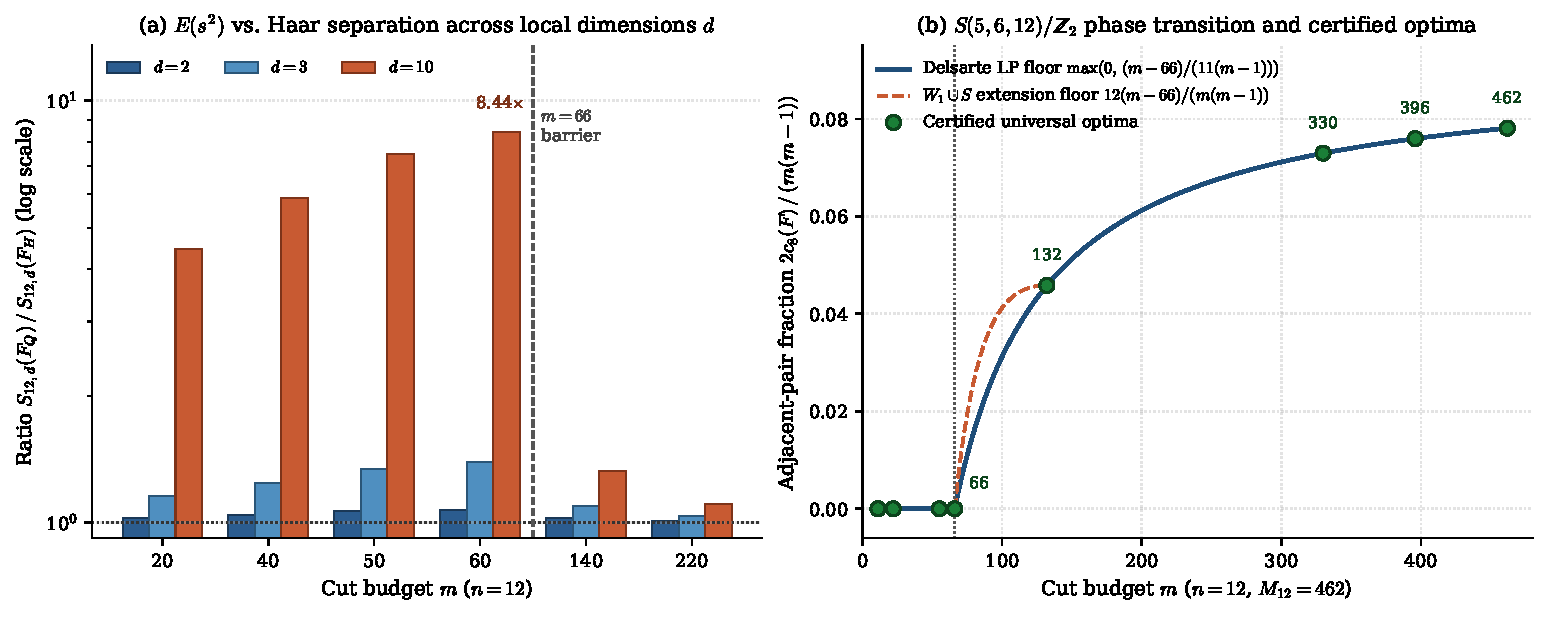
\includegraphics[width=0.98\textwidth]{figures/fig1_es2_vs_haar_n12.pdf}
\caption{Overbudget geometry at $n=12$: (a) separation ratio $S_{12,d}(\F_Q)/S_{12,d}(\F_H)$ across $d \in \{2,3,10\}$ peaking at $8.44\times$ before the $m=66$ barrier; (b) Delsarte LP floor for the adjacent-pair fraction $2c_8(\F)/(m(m-1))$, the $W_1 \cup S$ extension wall, and the eight certified universal optima from Table~\ref{tab:n12_optima}.}
\label{fig:n12_phase}
\end{figure}

\section{Asymptotic Collapse and Parseval Sandwich Bounds}\label{sec:asymptotics}

In the high-budget regime, spectral positivity of $\Jbar(2k,k)$ locks the global minimum tightly between the $i=0$ harmonic floor and the random-subset upper bound.

\begin{proof}[Proof of Theorem~\ref{thm:asymptotic}]
By Theorem~\ref{thm:spectral} at $i=0$, $R_{n,d} = \Lambda_0(n,d) = \sum_{r=0}^k (d^2-1)^r \binom{k}{k-r}\binom{2k-r}{k-r}$. More directly, summing $h_{n,d}(g_{AB}) = d^{2q} + d^{2(k-q)}$ over all folded vertices $\{B, B^c\}$ around a fixed $A$ gives
\[
R_{n,d} = \frac{1}{2}\sum_{B \in \binom{[2k]}{k}} \bigl(d^{2|A\cap B|} + d^{2(k-|A\cap B|)}\bigr) = \sum_{q=0}^k \binom{k}{q}^2 d^{2q}.
\]
Applying Parseval's identity to $(d + e^{i\theta})^k (d + e^{-i\theta})^k = \bigl((d+1)^2 - 4d\sin^2(\theta/2)\bigr)^k$ yields the integral in~\eqref{eq:parseval}. As $k \to \infty$ with $d \ge 2$ fixed, $0 \le \frac{4d}{(d+1)^2}\sin^2(\theta/2) \le \frac{4d}{(d+1)^2} < 1$, so the integral concentrates in a $k^{-1/2}$-neighborhood of $\theta = 0$ where $1 - \frac{4d}{(d+1)^2}\sin^2(\theta/2) = \exp\bigl(-\frac{d}{(d+1)^2}\theta^2 + O(\theta^4)\bigr)$. Laplace's method gives
\[
R_{n,d} = \frac{(d+1)^{2k}}{2\pi}\sqrt{\frac{\pi(d+1)^2}{kd}}\bigl(1 + O(k^{-1})\bigr) = \frac{d+1}{\sqrt{d}}\left(\frac{d+1}{2}\right)^n \frac{2^n}{2\sqrt{\pi k}}\bigl(1 + O(k^{-1})\bigr).
\]
Dividing by Stirling's formula $M_n = \frac{1}{2}\binom{2k}{k} = \frac{2^n}{2\sqrt{\pi k}}(1 + O(k^{-1}))$ proves~\eqref{eq:parseval}.

For~(b), since $\|\Pi_0 \mathbf{1}_{\F}\|^2 = m^2/M_n$, expanding $\sum_{a,b \in \F} h_{n,d}(g_{ab}) = m(d^n + 1) + 2 S_{n,d}(\F)$ via Theorem~\ref{thm:spectral}(a) and discarding the nonnegative $i \ge 2$ terms ($\Lambda_i > 0$) yields $m(d^n + 1) + 2 S_{n,d}(\F) \ge \Lambda_0 \|\Pi_0 \mathbf{1}_{\F}\|^2 = \frac{m^2}{M_n} R_{n,d}$, proving the lower bound in~\eqref{eq:sandwich}. For the upper bound, averaging $S_{n,d}(\F)$ uniformly over all $\binom{M_n}{m}$ families of size $m$ gives $\E[S_{n,d}(\F)] = \binom{m}{2}\frac{M_n R_{n,d} - M_n(d^n+1)}{M_n(M_n-1)} = \frac{m(m-1)}{2(M_n-1)}(R_{n,d} - d^n - 1)$, so at least one family attains at most this value.

For~(c), once $m/M_n \gg \sqrt{n}\,(d/(d+1))^n$, we have $\frac{m}{M_n}R_{n,d} \gg d^n + 1$, so the $\max(0,\cdot)$ floor in~\eqref{eq:sandwich} is eventually inactive. Moreover, the gap between the upper and lower bounds in~\eqref{eq:sandwich} is bounded above by $\frac{m(M_n-m)}{2(M_n-1)}(d^n+1) \le \frac{m}{2}(d^n+1)$, while the leading lower-bound term $\frac{m^2}{2M_n} R_{n,d}$ satisfies
\[
\frac{m(d^n+1)}{\frac{m^2}{M_n} R_{n,d}} = \frac{M_n(d^n+1)}{m R_{n,d}} \asymp \frac{M_n}{m} \cdot \frac{\sqrt{n}\,(2d)^n}{(2(d+1))^n} = \frac{M_n}{m}\sqrt{n}\left(\frac{d}{d+1}\right)^n.
\]
Hence the relative gap vanishes as $o(1)$ under $m/M_n \gg \sqrt{n}\,(d/(d+1))^n$, and decays exponentially as $O\bigl(\rho^{-1}\sqrt{n}(d/(d+1))^n\bigr)$ when $m = \lfloor \rho M_n \rfloor$ for any fixed $\rho \in (0,1]$. Substituting $R_{n,d}/M_n = \frac{d+1}{\sqrt{d}}(\frac{d+1}{2})^n(1+o(1))$ completes the proof of~(c).
\end{proof}

Figure~\ref{fig:asymptotic} illustrates the exponential spectral hierarchy of Theorem~\ref{thm:spectral} alongside the $O(1/n)$ convergence of $R_{n,d}/M_n$ up to $n=320$.

\begin{figure}[htbp]
\centering
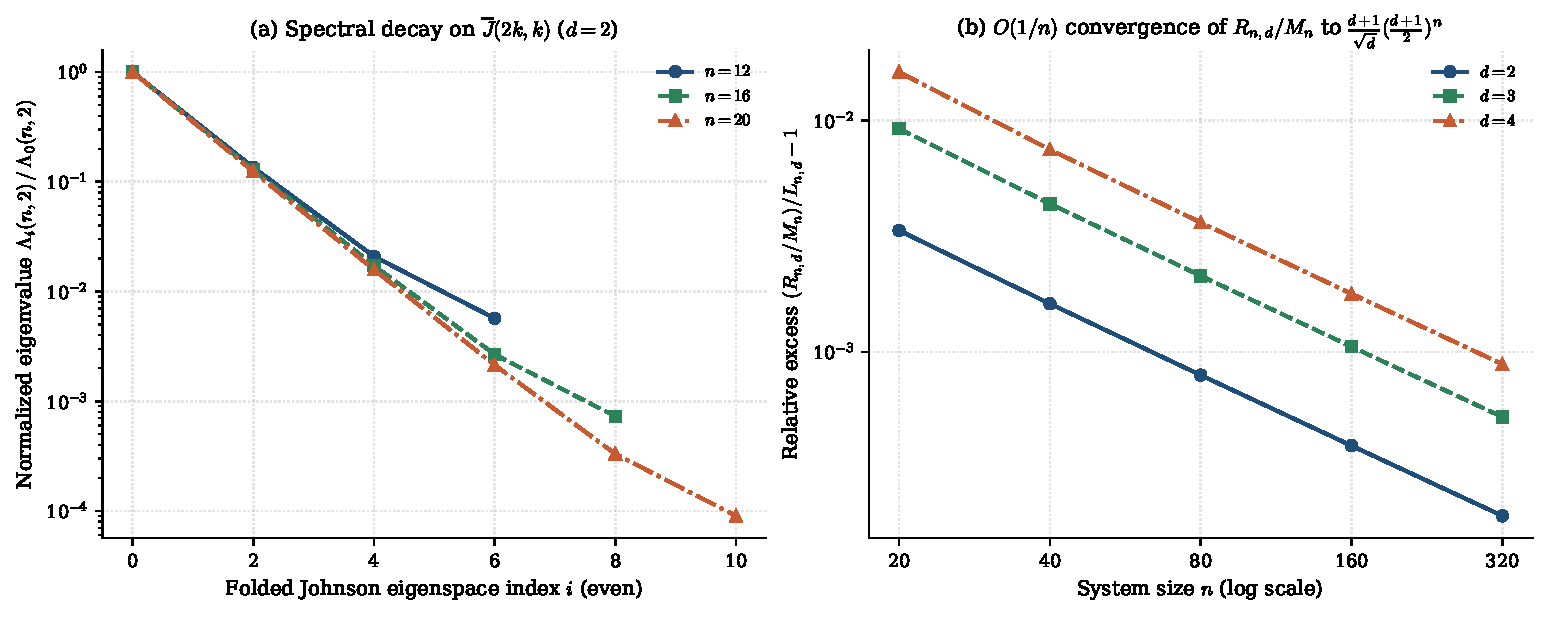
\includegraphics[width=0.98\textwidth]{figures/fig2_asymptotic_collapse.pdf}
\caption{(a) Normalized folded Johnson eigenvalues $\Lambda_i(n,2)/\Lambda_0(n,2)$ for $n \in \{12,16,20\}$; (b) $O(1/n)$ relative convergence of $R_{n,d}/M_n$ to $L_{n,d} := \frac{d+1}{\sqrt{d}}(\frac{d+1}{2})^n$ across $n \in \{20,40,80,160,320\}$ and $d \in \{2,3,4\}$.}
\label{fig:asymptotic}
\end{figure}

\section{Scope, Epistemic Separation, and Open Problems}\label{sec:open}

Following strict separation between unconditional theorems, finite certificates, and open questions:
\begin{enumerate}
\item \emph{Layer 1 (Unconditional analytic theorems):} Theorems~\ref{thm:separation}(a)--(b), \ref{thm:spectral}, \ref{thm:witt}(a)--(b), and~\ref{thm:asymptotic} hold globally via closed-form analytic proofs without computer assistance.
\item \emph{Layer 2 (Finite exact certificates):} Theorem~\ref{thm:separation}(c) (Table~\ref{tab:separation}) and Theorem~\ref{thm:witt}(c) (Table~\ref{tab:n12_optima}) rest on canonical bitmask witnesses archived in \url{scripts/certificates_data.json} and checked via exact rational and polynomial arithmetic in \url{scripts/verify_overbudget_designs.py}, which also independently verifies $S_4$ contractions ($k\in\{3,4,5\}$), folded Johnson spectra ($6 \le n \le 20$), Delsarte dual polynomials ($n \in \{12,14\}$), Golay/Witt exterior intersections, and five negative mutation checks in under one second ($0.87\,$s measured, $0.18\,$MB peak traced memory, zero floating-point relaxations). Notice that the separating pairs $(\F_Q, \F_H)$ in Table~\ref{tab:separation} are constructive witnesses of $Q(\F_Q) \le Q(\F_H)$ paired with $S_{n,d}(\F_Q) > S_{n,d}(\F_H)$, not claims of global optimality outside the certified parameters of Table~\ref{tab:n12_optima}.
\item \emph{Layer 3 (Open questions):} In the $3$-class scheme $\Jbar(12,6)$ (Theorem~\ref{thm:witt}(b)), strict spectral monotonicity ($\Lambda_0 > \Lambda_2 > \Lambda_4 > \Lambda_6 > 0$, Theorem~\ref{thm:spectral}(a)) yields $d$-uniform LP optimality both in the $2$-class ($\Pi_2 = 0$, $c_8 = 0$) regime and once $t=4$ ($\Pi_2 = \Pi_4 = 0$) binds. For larger schemes ($n \ge 16$) with additional free eigenspaces or non-vertex budgets $n < m < M_n$, whether the discrete integer minimizers can depend on $d$ remains open:
\end{enumerate}

\begin{problem}[Realizable dimension crossovers]\label{prob:crossover}
Does there exist an even system size $n \ge 12$, a cut budget $m$ with $n < m < M_n$, and distinct local dimensions $d_1 \ne d_2$ such that the exact integer minimizers of $S_{n,d_1}(\F)$ and $S_{n,d_2}(\F)$ over $|\F|=m$ are disjoint? Equivalently, where can the discrete feasible polytope break the dimension-invariance observed at the LP vertex and at $m=n$~\cite{Shiroshita2026}?
\end{problem}

\appendix

\section{Exact Asymptotic Prefactor Convergence Data}\label{app:asymp}

For independent verification of Theorem~\ref{thm:asymptotic}(a), Table~\ref{tab:app_asymp} records the normalized row-sum prefactor $P_n(d) := (R_{n,d}/M_n)\bigl(\frac{2}{d+1}\bigr)^n$ and relative excess $P_n(d)/L_d - 1$ computed from exact integers in \url{scripts/verify_overbudget_designs.py} toward $L_d := (d+1)/\sqrt{d}$.

\begin{table}[htbp]
\centering
\caption{Exact normalized Parseval prefactor $P_n(d) := (R_{n,d}/M_n)\bigl(\frac{2}{d+1}\bigr)^n$ and relative excess $P_n(d)/L_d - 1$ toward $L_d := (d+1)/\sqrt{d}$.}
\label{tab:app_asymp}
\footnotesize
\begin{tabular}{@{}rrrrrrr@{}}
\toprule
$n$ & $P_n(2)$ & Excess ($d=2$) & $P_n(3)$ & Excess ($d=3$) & $P_n(4)$ & Excess ($d=4$) \\
\midrule
$20$  & $2.12841809$ & $0.00334591$ & $2.33065370$ & $0.00920266$ & $2.54038774$ & $0.01615510$ \\
$40$  & $2.12474613$ & $0.00161493$ & $2.31947884$ & $0.00436380$ & $2.51869196$ & $0.00747678$ \\
$80$  & $2.12300478$ & $0.00079405$ & $2.31432159$ & $0.00213065$ & $2.50905141$ & $0.00362056$ \\
$160$ & $2.12215569$ & $0.00039379$ & $2.31183350$ & $0.00105327$ & $2.50445837$ & $0.00178335$ \\
$320$ & $2.12173633$ & $0.00019610$ & $2.31061053$ & $0.00052371$ & $2.50221302$ & $0.00088521$ \\
\midrule
$\infty$ & $2.12132034$ & $0$ & $2.30940108$ & $0$ & $2.50000000$ & $0$ \\
\bottomrule
\end{tabular}
\end{table}

\section*{Use of AI}
Portions of the computational exploration, exact Python verification scripts (\url{scripts/verify_overbudget_designs.py}, \url{scripts/generate_figures.py}), figure formatting, and LaTeX preparation were assisted by Google DeepMind's Gemini AI system. All mathematical claims, derivations, and numerical certificates were independently audited, cross-checked with exact rational and polynomial arithmetic, and validated by the author.

\bibliographystyle{plainnat}
\bibliography{references}

\end{document}
